\documentclass{beamer}
\usepackage{graphicx}

% Theme
%\usetheme{CambridgeUS}
\usetheme{metropolis}  


%Package
\usepackage[linesnumbered,ruled,vlined]{algorithm2e}
\usepackage{tikz}
\usepackage{multicol}
\usepackage{mdframed}
\usepackage[T1]{fontenc}

%templete
\newmdenv[linecolor=black,linewidth=1pt]{mybox}
\setbeamertemplate{section in toc}[sections numbered]
\setbeamertemplate{subsection in toc}[subsections numbered]


% Title page
\title{Insertion and Selection Sort}
%\subtitle{Group Name}
\author{
  \begin{tabular}{ccc}
    Md. Abu Sufyan & Tameem Rahman & Partha Paul \\
    Roll: 2003085 & Roll: 2003089 & Roll: 2003078 \\
    Department: CSE & Department: CSE & Department: CSE \\
    \\
    Atik Mohtasin Rahi & Barkatulla Barik & Mir Ashikur Rahman \\
    Roll: 2003118 & Roll: 2003071 & Roll: 2003109 \\
    Department: CSE & Department: CSE & Department: CSE
  \end{tabular}
}


% Begin document
\begin{document}

\begin{frame}
  \titlepage
\end{frame}


% Welcome slide
\section{Welcome}
\begin{frame}{Welcome}
  \begin{center}
    \Huge Welcome to our Presentation!
  \end{center}
\end{frame}

% Outline slide
\begin{frame}[shrink=15]{Outline}
    \begin{multicols}{2}
        \tableofcontents[hideallsubsections, sectionstyle=show, subsectionstyle=show]
    \end{multicols}
\end{frame}


\section{First Topic}
\begin{frame}{Selection Sort Overview}
  \begin{center}
    \Huge Selection Sort
  \end{center}
\end{frame}


\subsection{Selection sort First Pass}
\begin{frame}[c, fragile]
\frametitle{Selection Sort: First Pass}

\begin{itemize}
    \item For the first position in the sorted array, traverse the entire array.
    \item Find the minimum value (11) and swap it with the element at the first position (64).
\end{itemize}

\[
\begin{array}{c}
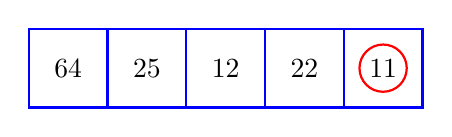
\begin{tikzpicture}[baseline=(current bounding box.center)]
    \node at (0,0) {64};
    \node at (1,0) {25};
    \node at (2,0) {12};
    \node at (3,0) {22};
    \node at (4,0) {11};
    \draw[red, thick] (4,0) circle (0.3);
    \draw[blue, thick] (-0.5,-0.5) rectangle (0.5,0.5);
    \draw[blue, thick] (0.5,-0.5) rectangle (1.5,0.5);
    \draw[blue, thick] (1.5,-0.5) rectangle (2.5,0.5);
    \draw[blue, thick] (2.5,-0.5) rectangle (3.5,0.5);
    \draw[blue, thick] (3.5,-0.5) rectangle (4.5,0.5);
\end{tikzpicture} \\
\downarrow \\
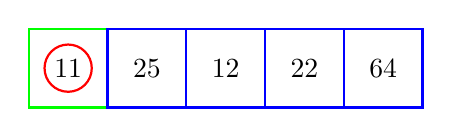
\begin{tikzpicture}[baseline=(current bounding box.center)]
    \node at (0,0) {11};
    \node at (1,0) {25};
    \node at (2,0) {12};
    \node at (3,0) {22};
    \node at (4,0) {64};
    \draw[red, thick] (0,0) circle (0.3);
    \draw[green, thick] (-0.5,-0.5) rectangle (0.5,0.5);
    \draw[blue, thick] (0.5,-0.5) rectangle (1.5,0.5);
    \draw[blue, thick] (1.5,-0.5) rectangle (2.5,0.5);
    \draw[blue, thick] (2.5,-0.5) rectangle (3.5,0.5);
    \draw[blue, thick] (3.5,-0.5) rectangle (4.5,0.5);
\end{tikzpicture}
\end{array}
\]

\end{frame}

\subsection{Selection Sort: Second Pass}
\begin{frame}[c, fragile]
\frametitle{Selection Sort: Second Pass}

\begin{itemize}
    \item For the second position, find the second minimum value (12) and swap it with the element at the second position (25).
\end{itemize}

\[
\begin{array}{c}
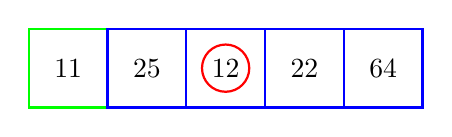
\begin{tikzpicture}[baseline=(current bounding box.center)]
    \node at (0,0) {11};
    \node at (1,0) {25};
    \node at (2,0) {12};
    \node at (3,0) {22};
    \node at (4,0) {64};
    \draw[red, thick] (2,0) circle (0.3);
    \draw[green, thick] (-0.5,-0.5) rectangle (0.5,0.5);
    \draw[blue, thick] (0.5,-0.5) rectangle (1.5,0.5);
    \draw[blue, thick] (1.5,-0.5) rectangle (2.5,0.5);
    \draw[blue, thick] (2.5,-0.5) rectangle (3.5,0.5);
    \draw[blue, thick] (3.5,-0.5) rectangle (4.5,0.5);
\end{tikzpicture} \\
\downarrow \\
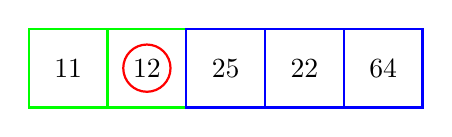
\begin{tikzpicture}[baseline=(current bounding box.center)]
    \node at (0,0) {11};
    \node at (1,0) {12};
    \node at (2,0) {25};
    \node at (3,0) {22};
    \node at (4,0) {64};
    \draw[red, thick] (1,0) circle (0.3);
    \draw[green, thick] (-0.5,-0.5) rectangle (0.5,0.5);
    \draw[green, thick] (0.5,-0.5) rectangle (1.5,0.5);
    \draw[blue, thick] (1.5,-0.5) rectangle (2.5,0.5);
    \draw[blue, thick] (2.5,-0.5) rectangle (3.5,0.5);
    \draw[blue, thick] (3.5,-0.5) rectangle (4.5,0.5);
\end{tikzpicture}
\end{array}
\]

\end{frame}

\subsection{Selection Sort: Third Pass}
\begin{frame}[c, fragile]
\frametitle{Selection Sort: Third Pass}

\begin{itemize}
    \item For the third position, find the third minimum value (22) and swap it with the element at the third position (25).
\end{itemize}

\[
\begin{array}{c}
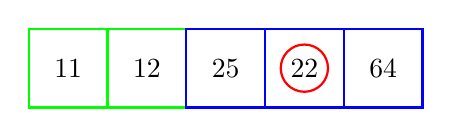
\begin{tikzpicture}[baseline=(current bounding box.center)]
    \node at (0,0) {11};
    \node at (1,0) {12};
    \node at (2,0) {25};
    \node at (3,0) {22};
    \node at (4,0) {64};
    \draw[red, thick] (3,0) circle (0.3);
    \draw[green, thick] (-0.5,-0.5) rectangle (0.5,0.5);
    \draw[green, thick] (0.5,-0.5) rectangle (1.5,0.5);
    \draw[blue, thick] (1.5,-0.5) rectangle (2.5,0.5);
    \draw[blue, thick] (2.5,-0.5) rectangle (3.5,0.5);
    \draw[blue, thick] (3.5,-0.5) rectangle (4.5,0.5);
\end{tikzpicture} \\
\downarrow \\
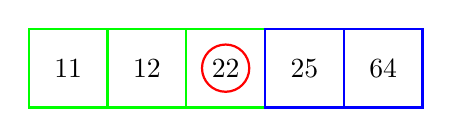
\begin{tikzpicture}[baseline=(current bounding box.center)]
    \node at (0,0) {11};
    \node at (1,0) {12};
    \node at (2,0) {22};
    \node at (3,0) {25};
    \node at (4,0) {64};
    \draw[red, thick] (2,0) circle (0.3);
    \draw[green, thick] (-0.5,-0.5) rectangle (0.5,0.5);
    \draw[green, thick] (0.5,-0.5) rectangle (1.5,0.5);
    \draw[green, thick] (1.5,-0.5) rectangle (2.5,0.5);
    \draw[blue, thick] (2.5,-0.5) rectangle (3.5,0.5);
    \draw[blue, thick] (3.5,-0.5) rectangle (4.5,0.5);
\end{tikzpicture} 
\end{array}
\]

\end{frame}

\subsection{Selection Sort: Fourth Pass}
\begin{frame}[c, fragile]
\frametitle{Selection Sort: Fourth Pass}

\begin{itemize}
    \item For the fourth position, find the fourth minimum value (25) and never swap it.
\end{itemize}

\[
\begin{array}{c}
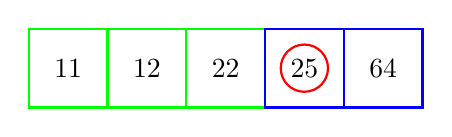
\begin{tikzpicture}[baseline=(current bounding box.center)]
    \node at (0,0) {11};
    \node at (1,0) {12};
    \node at (2,0) {22};
    \node at (3,0) {25};
    \node at (4,0) {64};
    \draw[red, thick] (3,0) circle (0.3);
    \draw[green, thick] (-0.5,-0.5) rectangle (0.5,0.5);
    \draw[green, thick] (0.5,-0.5) rectangle (1.5,0.5);
    \draw[green, thick] (1.5,-0.5) rectangle (2.5,0.5);
    \draw[blue, thick] (2.5,-0.5) rectangle (3.5,0.5);
    \draw[blue, thick] (3.5,-0.5) rectangle (4.5,0.5);
\end{tikzpicture}  \\
\downarrow \\
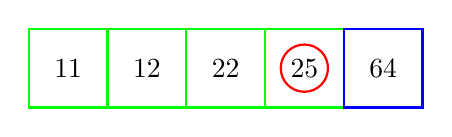
\begin{tikzpicture}[baseline=(current bounding box.center)]
    \node at (0,0) {11};
    \node at (1,0) {12};
    \node at (2,0) {22};
    \node at (3,0) {25};
    \node at (4,0) {64};
    \draw[red, thick] (3,0) circle (0.3);
    \draw[green, thick] (-0.5,-0.5) rectangle (0.5,0.5);
    \draw[green, thick] (0.5,-0.5) rectangle (1.5,0.5);
    \draw[green, thick] (1.5,-0.5) rectangle (2.5,0.5);
    \draw[green, thick] (2.5,-0.5) rectangle (3.5,0.5);
    \draw[blue, thick] (3.5,-0.5) rectangle (4.5,0.5);
\end{tikzpicture}
\end{array}
\]

\end{frame}

\subsection{Selection Sort: Fifth Pass}
\begin{frame}[c, fragile]
\frametitle{Selection Sort: Fifth Pass}

\begin{itemize}
    \item The largest value (64) is automatically placed at the last position.
\end{itemize}

\[
\begin{array}{c}
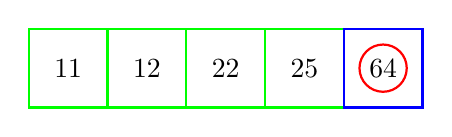
\begin{tikzpicture}[baseline=(current bounding box.center)]
    \node at (0,0) {11};
    \node at (1,0) {12};
    \node at (2,0) {22};
    \node at (3,0) {25};
    \node at (4,0) {64};
    \draw[red, thick] (4,0) circle (0.3);
    \draw[green, thick] (-0.5,-0.5) rectangle (0.5,0.5);
    \draw[green, thick] (0.5,-0.5) rectangle (1.5,0.5);
    \draw[green, thick] (1.5,-0.5) rectangle (2.5,0.5);
    \draw[green, thick] (2.5,-0.5) rectangle (3.5,0.5);
    \draw[blue, thick] (3.5,-0.5) rectangle (4.5,0.5);
\end{tikzpicture} \\
\downarrow \\
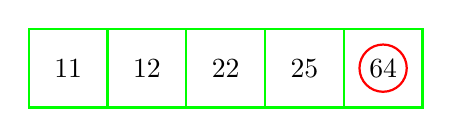
\begin{tikzpicture}[baseline=(current bounding box.center)]
    \node at (0,0) {11};
    \node at (1,0) {12};
    \node at (2,0) {22};
    \node at (3,0) {25};
    \node at (4,0) {64};
    \draw[red, thick] (4,0) circle (0.3);
    \draw[green, thick] (-0.5,-0.5) rectangle (0.5,0.5);
    \draw[green, thick] (0.5,-0.5) rectangle (1.5,0.5);
    \draw[green, thick] (1.5,-0.5) rectangle (2.5,0.5);
    \draw[green, thick] (2.5,-0.5) rectangle (3.5,0.5);
    \draw[green, thick] (3.5,-0.5) rectangle (4.5,0.5);
\end{tikzpicture}
\end{array}
\]

\end{frame}

% Welcome slide
\subsection{Selection Sort Algorithm}
\begin{frame}[fragile]
\frametitle{Selection Sort Algorithm}


\begin{algorithm}[H]
\caption{Selection Sort}
\label{algo:selectionsort}
\KwData{Array $arr$ of size $n$}
\KwResult{Sorted array $arr$}

\For{$i \leftarrow 0$ \KwTo $n-1$}{
    $min\_idx \leftarrow i$\;
    \For{$j \leftarrow i + 1$ \KwTo $n$}{
        \If{$arr[j] < arr[min\_idx]$}{
            $min\_idx \leftarrow j$\;
        }
    }
    \If{$min\_idx \neq i$}{
        Swap($arr[min\_idx]$, $arr[i]$)\;
    }
}
\end{algorithm}

\end{frame}


\begin{frame}[c, fragile]
\frametitle{Selection Sort: C++ Code}

\begin{mybox}  % Use the newly defined box environment
\begin{verbatim}
void selectionSort(int arr[], int n) 
{ 
    int i, j, min_idx; 
    for (i = 0; i < n - 1; i++) { 
        min_idx = i; 
        for (j = i + 1; j < n; j++) { 
            if (arr[j] < arr[min_idx]) 
                min_idx = j; 
        } 
        if (min_idx != i) 
            swap(arr[min_idx], arr[i]); 
    } 
}
\end{verbatim}
\end{mybox}

\end{frame}

\section{Second Topic}
\begin{frame}{Insertion Sort}
  \begin{center}
    \Huge Insertion Sort
  \end{center}
\end{frame}

\subsection{Insertion Sort Steps}
\begin{frame}[c, fragile]
  \frametitle{Insertion Sort: Step-by-Step}

  \begin{itemize}
    \item For each element, insert it into its correct position in the sorted portion of the array.
    \item Shift elements greater than the key to the right.
    \item Repeat until the entire array is sorted.
  \end{itemize}

\end{frame}

\subsection{Insertion sort First Pass}
\begin{frame}[c, fragile]
\frametitle{Insertion Sort: First Pass}

\begin{itemize}
    \item Initially, the first two elements of the array are compared in insertion sort.
    \item Here, 23 is greater than 1 hence they are not in the ascending order and 23 is not at its correct position. Thus, swap 1 and 23.
\end{itemize}

\[
\begin{array}{c}
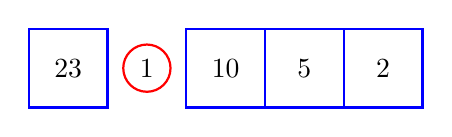
\begin{tikzpicture}[baseline=(current bounding box.center)]
    \node at (0,0) {23};
    \node at (1,0) {1};
    \node at (2,0) {10};
    \node at (3,0) {5};
    \node at (4,0) {2};
    \draw[red, thick] (1,0) circle (0.3);
    \draw[blue, thick] (-0.5,-0.5) rectangle (0.5,0.5);
    \draw[blue, thick] (1.5,-0.5) rectangle (2.5,0.5);
    \draw[blue, thick] (2.5,-0.5) rectangle (3.5,0.5);
    \draw[blue, thick] (3.5,-0.5) rectangle (4.5,0.5);
\end{tikzpicture} \\
\downarrow \\
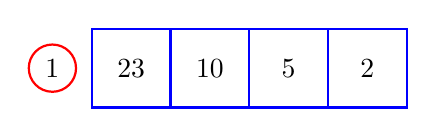
\begin{tikzpicture}[baseline=(current bounding box.center)]
    \node at (0,0) {1};
    \node at (1,0) {23};
    \node at (2,0) {10};
    \node at (3,0) {5};
    \node at (4,0) {2};
    \draw[red, thick] (0,0) circle (0.3);
    \draw[blue, thick] (0.5,-0.5) rectangle (1.5,0.5);
    \draw[blue, thick] (1.5,-0.5) rectangle (2.5,0.5);
    \draw[blue, thick] (2.5,-0.5) rectangle (3.5,0.5);
    \draw[blue, thick] (3.5,-0.5) rectangle (4.5,0.5);
\end{tikzpicture}
\end{array}
\]
\end{frame}

\subsection{Insertion sort Second Pass}
\begin{frame}[c, fragile]
\frametitle{Insertion Sort: Second Pass}

\begin{itemize}
    \item Here, 23 is greater than 10 hence they are not in the ascending order and 10 is not at its correct position. Thus, swap 1 and 23. 10 also stored in a sorted sub-array along with 1
\end{itemize}

\[
\begin{array}{c}
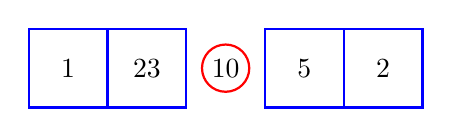
\begin{tikzpicture}[baseline=(current bounding box.center)]
    \node at (0,0) {1};
    \node at (1,0) {23};
    \node at (2,0) {10};
    \node at (3,0) {5};
    \node at (4,0) {2};
    \draw[red, thick] (2,0) circle (0.3);
    \draw[blue, thick] (-0.5,-0.5) rectangle (0.5,0.5);
    \draw[blue, thick] (0.5,-0.5) rectangle (1.5,0.5);
    \draw[blue, thick] (2.5,-0.5) rectangle (3.5,0.5);
    \draw[blue, thick] (3.5,-0.5) rectangle (4.5,0.5);
\end{tikzpicture} \\
\downarrow \\
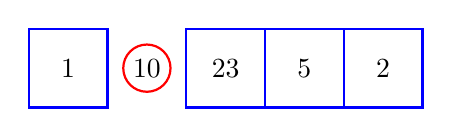
\begin{tikzpicture}[baseline=(current bounding box.center)]
    \node at (0,0) {1};
    \node at (1,0) {10};
    \node at (2,0) {23};
    \node at (3,0) {5};
    \node at (4,0) {2};
    \draw[red, thick] (1,0) circle (0.3);
    \draw[blue, thick] (-0.5,-0.5) rectangle (0.5,0.5);
    \draw[blue, thick] (1.5,-0.5) rectangle (2.5,0.5);
    \draw[blue, thick] (2.5,-0.5) rectangle (3.5,0.5);
    \draw[blue, thick] (3.5,-0.5) rectangle (4.5,0.5);
\end{tikzpicture}
\end{array}
\]
\end{frame}

\subsection{Insertion sort Third Pass}
\begin{frame}[c, fragile]
\frametitle{Insertion Sort: Third Pass}

\begin{itemize}
    \item Here, 5 isn't in correct position. So 5 has to be swapped with its previous position until 5 isn't greater than the previous value.
\end{itemize}

\[
\begin{array}{c}
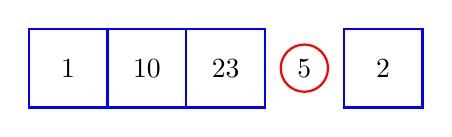
\begin{tikzpicture}[baseline=(current bounding box.center)]
    \node at (0,0) {1};
    \node at (1,0) {10};
    \node at (2,0) {23};
    \node at (3,0) {5};
    \node at (4,0) {2};
    \draw[red, thick] (3,0) circle (0.3);
    \draw[blue, thick] (-0.5,-0.5) rectangle (0.5,0.5);
    \draw[blue, thick] (0.5,-0.5) rectangle (1.5,0.5);
    \draw[blue, thick] (1.5,-0.5) rectangle (2.5,0.5);
    \draw[blue, thick] (3.5,-0.5) rectangle (4.5,0.5);
\end{tikzpicture} \\
\downarrow \\
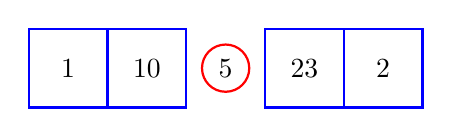
\begin{tikzpicture}[baseline=(current bounding box.center)]
    \node at (0,0) {1};
    \node at (1,0) {10};
    \node at (2,0) {5};
    \node at (3,0) {23};
    \node at (4,0) {2};
    \draw[red, thick] (2,0) circle (0.3);
    \draw[blue, thick] (-0.5,-0.5) rectangle (0.5,0.5);
    \draw[blue, thick] (0.5,-0.5) rectangle (1.5,0.5);
    \draw[blue, thick] (2.5,-0.5) rectangle (3.5,0.5);
    \draw[blue, thick] (3.5,-0.5) rectangle (4.5,0.5);
\end{tikzpicture} \\
\downarrow \\
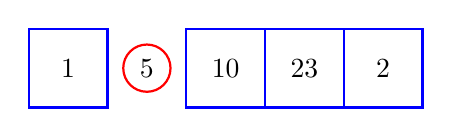
\begin{tikzpicture}[baseline=(current bounding box.center)]
    \node at (0,0) {1};
    \node at (1,0) {5};
    \node at (2,0) {10};
    \node at (3,0) {23};
    \node at (4,0) {2};
    \draw[red, thick] (1,0) circle (0.3);
    \draw[blue, thick] (-0.5,-0.5) rectangle (0.5,0.5);
    \draw[blue, thick] (1.5,-0.5) rectangle (2.5,0.5);
    \draw[blue, thick] (2.5,-0.5) rectangle (3.5,0.5);
    \draw[blue, thick] (3.5,-0.5) rectangle (4.5,0.5);
\end{tikzpicture}
\end{array}
\]
\end{frame}

\subsection{Insertion sort Fourth Pass}
\begin{frame}[c, fragile]
\frametitle{Insertion Sort: Fourth Pass}

\begin{itemize}
    \item Here, 2 isn't in correct position. To place 2 in correct position, we have to follow the same procedure as third pass.
\end{itemize}

\[
\begin{array}{c}
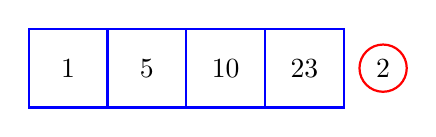
\begin{tikzpicture}[baseline=(current bounding box.center)]
    \node at (0,0) {1};
    \node at (1,0) {5};
    \node at (2,0) {10};
    \node at (3,0) {23};
    \node at (4,0) {2};
    \draw[red, thick] (4,0) circle (0.3);
    \draw[blue, thick] (-0.5,-0.5) rectangle (0.5,0.5);
    \draw[blue, thick] (0.5,-0.5) rectangle (1.5,0.5);
    \draw[blue, thick] (1.5,-0.5) rectangle (2.5,0.5);
    \draw[blue, thick] (2.5,-0.5) rectangle (3.5,0.5);
\end{tikzpicture} \\
\downarrow \\
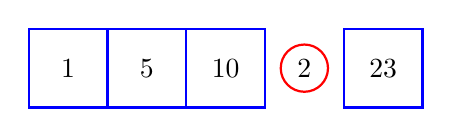
\begin{tikzpicture}[baseline=(current bounding box.center)]
    \node at (0,0) {1};
    \node at (1,0) {5};
    \node at (2,0) {10};
    \node at (3,0) {2};
    \node at (4,0) {23};
    \draw[red, thick] (3,0) circle (0.3);
    \draw[blue, thick] (-0.5,-0.5) rectangle (0.5,0.5);
    \draw[blue, thick] (0.5,-0.5) rectangle (1.5,0.5);
    \draw[blue, thick] (1.5,-0.5) rectangle (2.5,0.5);
    \draw[blue, thick] (3.5,-0.5) rectangle (4.5,0.5);
\end{tikzpicture} \\
\downarrow \\
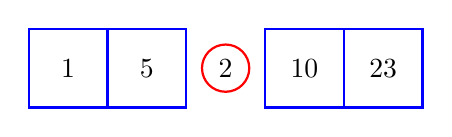
\begin{tikzpicture}[baseline=(current bounding box.center)]
    \node at (0,0) {1};
    \node at (1,0) {5};
    \node at (2,0) {2};
    \node at (3,0) {10};
    \node at (4,0) {23};
    \draw[red, thick] (2,0) circle (0.3);
    \draw[blue, thick] (-0.5,-0.5) rectangle (0.5,0.5);
    \draw[blue, thick] (0.5,-0.5) rectangle (1.5,0.5);
    \draw[blue, thick] (2.5,-0.5) rectangle (3.5,0.5);
    \draw[blue, thick] (3.5,-0.5) rectangle (4.5,0.5);
\end{tikzpicture} \\
\downarrow \\
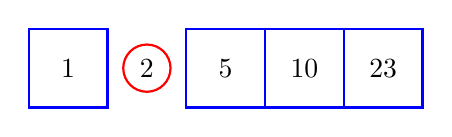
\begin{tikzpicture}[baseline=(current bounding box.center)]
    \node at (0,0) {1};
    \node at (1,0) {2};
    \node at (2,0) {5};
    \node at (3,0) {10};
    \node at (4,0) {23};
    \draw[red, thick] (1,0) circle (0.3);
    \draw[blue, thick] (-0.5,-0.5) rectangle (0.5,0.5);
    \draw[blue, thick] (1.5,-0.5) rectangle (2.5,0.5);
    \draw[blue, thick] (2.5,-0.5) rectangle (3.5,0.5);
    \draw[blue, thick] (3.5,-0.5) rectangle (4.5,0.5);
\end{tikzpicture}
\end{array}
\]
\end{frame}

\subsection{Insertion Sort Demonstration}
\begin{frame}[c, fragile]
  \frametitle{Insertion Sort: Visualization}

  \begin{figure}
    \centering
    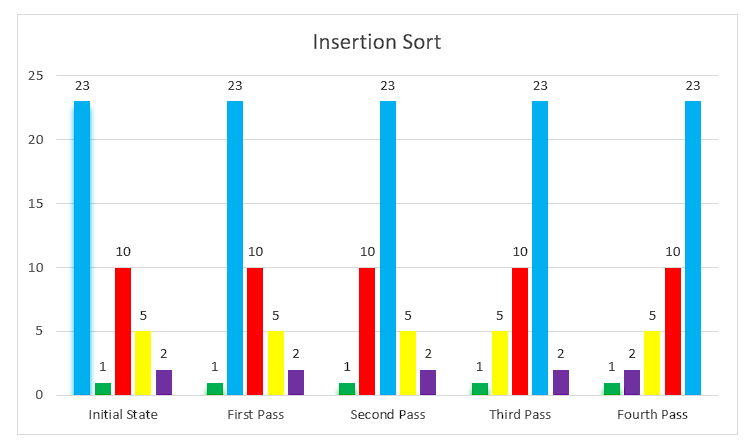
\includegraphics[width=0.7\textwidth]{chart2.png}
    \caption{Insertion Sort Visualization}
    \label{fig:insertion-visualization}
  \end{figure}

\end{frame}

\subsection{Insertion Sort Algorithm}
\begin{frame}[fragile]
  \frametitle{Insertion Sort Algorithm: Overview}
   \begin{algorithm}[H]
    \caption{Insertion Sort}
    \label{algo:insertionsort}
    \KwData{Array $arr$ of size $n$}
    \KwResult{Sorted array $arr$}

    \For{$i \leftarrow 1$ \KwTo $n$}{
      $key \leftarrow arr[i]$\;
      $j \leftarrow i - 1$\;
      \While{$j \geq 0$ \textbf{and} $arr[j] > key$}{
        $arr[j + 1] \leftarrow arr[j]$\;
        $j \leftarrow j - 1$\;
      }
      $arr[j + 1] \leftarrow key$\;
    }
  \end{algorithm}  
 

\end{frame}

\subsection{Insertion Sort C++ Code}
\begin{frame}[fragile]
  \frametitle{Insertion Sort: C++ Code}
  
\begin{mybox}
\begin{verbatim}
void insertionSort(int arr[], int n) {
    for (int i = 1; i < n; i++) {
        int key = arr[i];
        int j = i - 1;

        while (j >= 0 && arr[j] > key) {
            arr[j + 1] = arr[j];
            j = j - 1;
        }

        arr[j + 1] = key;
    }
}
\end{verbatim} 
\end{mybox}


\end{frame}


\section{Result \& Complexity Analysis}
\begin{frame}{Result and Complexity Analysis}
\begin{table}[H]
    \centering
    \small
    \captionsetup
    \label{tab:sort-comparison}
    \begin{tabular}{@{}S[table-format=6.0]SS[table-format=3.6]S[table-format=3.6]@{}}
        \toprule
        \textbf{Size} & \textbf{Insertion (s)} & \textbf{Selection (s)} \\
        \midrule
        10 & 0.000011 & 0.000019 \\
        50 & 0.000176 & 0.000155 \\
        100 & 0.000412 & 0.000363 \\
        500 & 0.004555 & 0.004457 \\
        1000 & 0.020648 & 0.018857 \\
        5000 & 0.528669 & 0.485517 \\
        10000 & 2.105405 & 1.965638 \\
        50000 &  61.877976 & 55.541591 \\
        100000  & 238.821475 & 271.276342\\
        \bottomrule
    \end{tabular}
    \captionsetup
    \caption{Performance Comparison of Insertion Sort and Selection Sort}
\end{table}
\end{frame}

\subsection{Graph}
\begin{frame}{Graph with Explanation}
  \begin{columns}
    \begin{column}{0.5\textwidth}
      \textbf{Explanation:}
      \begin{itemize}
        \item Point 1
        \item Point 2
        \item Point 3
      \end{itemize}
    \end{column}
    \begin{column}{0.5\textwidth}
      \begin{figure}
        \centering
        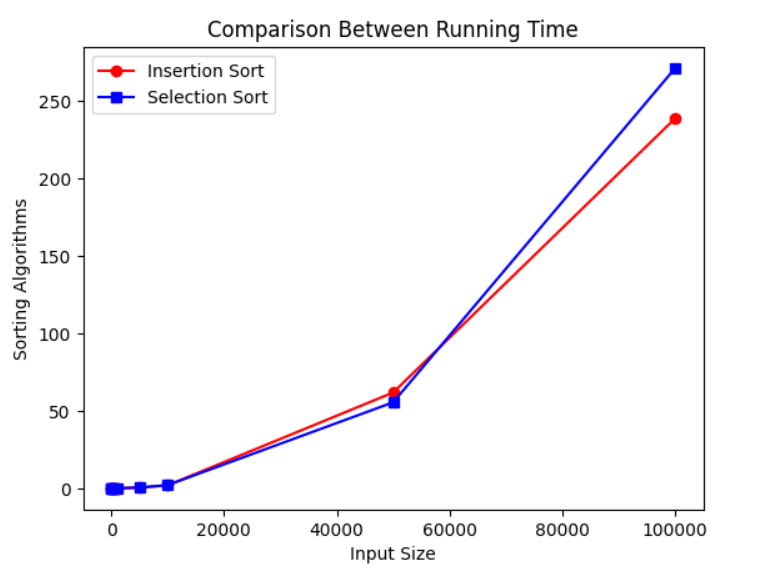
\includegraphics[width=\textwidth]{table1.png} % Replace 'example-image' with your actual image file name
        \caption{Complexity Graph.}
      \end{figure}
    \end{column}
  \end{columns}
\end{frame}

% References Slide
\section{References}
\begin{frame}[shrink=20]{References}
    \nocite{*} 
    \bibliographystyle{plain}
    \bibliography{Bibliography}
\end{frame}



\section{Conclusion}
\begin{frame}{Conclusion}
  \begin{itemize}
    \item Insertion Sort is a simple and intuitive sorting algorithm.
    \item It efficiently builds the final sorted array one element at a time.
    \item While not as efficient on large datasets as more advanced algorithms, it performs well on small datasets or nearly sorted datasets.
  \end{itemize}
\end{frame}

% Q&A Slide
\section{Questions \& Answers}
\begin{frame}{Questions \& Answers}
  \begin{center}
    \Huge Any Questions?
  \end{center}
\end{frame}

% Thanks Slide
\section{Thanks of all}


\end{document}
